%\documentclass[handout]{beamer} 
\documentclass[t,12pt,numbers,fleqn]{beamer}
%\documentclass[ignorenonframetext]{beamer}

\newif\ifquestions
%\questionstrue
\questionsfalse

\usepackage{pgfpages} 
\usepackage{hyperref}
\hypersetup{colorlinks=true,
    linkcolor=blue,
    citecolor=blue,
    filecolor=blue,
    urlcolor=blue,
    unicode=false}
\urlstyle{same}
\usepackage{listings}

\bibliographystyle{plain}

%\usetheme{Iimenau}

\useoutertheme{split} %so the footline can be seen, without needing pgfpages

%\pgfpagesuselayout{resize to}[letterpaper,border shrink=5mm,landscape]  %if this is uncommented, the hyperref links do not work

\mode<presentation>{}

\input{../def-beamer}

\newcommand{\topic}{09 Verification and Validation}

%Title page information for 1D04 lectures slides

% Define year specific parameters - used in title page and footer

\newcommand{\season}{Fall} %use to switch between Winter and Fall
\newcommand{\instructor}{Dr.~Spencer Smith} %use to switch instructor
\newcommand{\instructSmall}{Dr.~Smith}
\newcommand{\yr}{2019}
\newcommand{\courseCode}{CAS 741, CES 741}
\newcommand{\courseTitle}{Development of Scientific Computing Software}

%\setbeamerfont{structure}{series=\bfseries}
%\usefonttheme[stillsansseriftext,stillsansserifmath]{serif}
\setbeamertemplate{navigation symbols}{} 
\setbeamertemplate{itemize item}[ball]

\title{
  {\normalsize \bf 
    \borange{\courseCode~(\courseTitle)\\ \season~\yr}}\\[2ex]
  {\Large \bf \topic}}

\author[Smith]{\instructor}

\institute{
  Faculty of Engineering,
  McMaster University}

\date{
\today
%January 2011\\
\bc
  \includegraphics[scale = 0.2, keepaspectratio]
  {../mcmaster-logo-full-color.jpg}
\ec
}

\renewcommand{\borange}[1] %orange is too hard to read
{
   \bred{#1}
}

\begin{document}

\input{../footline}

%%%%%%%%%%%%%%%%%%%%%%%%%%%%%%%%%%%%%%%%%%%%%%%%%%%%%%

\begin{frame}
\frametitle{Verification and Validation}

\bi
\item Administrative details
\item Questions?
\item 741 workflow
\item Testing from SE perspective
\item Testing from SC perspective
\item V\&V template
\item V\&V examples
\bi
\item SWHS
\item Mesh Gen
\item Rogue Reborn
\ei
\ei
\end{frame}

%%%%%%%%%%%%%%%%%%%%%%%%%%%%%%%%%%%%%%%%%%%%%%%%%%%%%%

\begin{frame}
\frametitle{Administrative Details}

\bi
\item SRS Presentation grades on Avenue
\item Apology that unable to review full SRS
\item GitHub issues for colleagues
\bi
\item Assigned 1 colleague (see \texttt{Repos.xlsx} in repo)
\item Provide at least 5 issues on their SRS
\item Grading
\bi
\item Not enough issues, or poor issues 0/2
\item Enough issues, but shallow 1/2
\item Enough issues and deep (not surface) 2/2
\ei
\item Due by Tuesday, Oct 10, 11:59 pm
\ei
\item Reading week next week, no 741 classes
\item V\&V template updated in repo
\ei

\end{frame}

%%%%%%%%%%%%%%%%%%%%%%%%%%%%%%%%%%%%%%%%%%%%%%%%%%%%%%

\begin{frame}
\frametitle{Administrative Details: Deadlines}
~\newline
\begin{tabular}{l l l}
\textbf{SRS} & Week 05 & Oct 4\\
\textbf{SRS Issues} & Reading week & Oct 10\\
\textbf{V\&V Present} & Week 06 & Week of Oct 16\\
\textbf{V\&V Plan} & Week 07 & Oct 25\\
MG Present & Week 08 & Week of Oct 30\\
MG & Week 09 & Nov 8\\
MIS Present & Week 10 & Week of Nov 13\\
MIS & Week 11 & Nov 22\\
Impl.\ Present & Week 12 & Week of Nov 27\\
Final Documentation & Week 13 & Dec 6\\
\end {tabular}

\end{frame}

%%%%%%%%%%%%%%%%%%%%%%%%%%%%%%%%%%%%%%%%%%%%%%%%%%%%%%

\begin{frame}
\frametitle{Administrative Details: Presentation Schedule}

\bi
\item V\&V Present
\bi
\item \textbf{Tuesday: Steven, Alexandre P., Alexander S.}
\item \textbf{Friday: Geneva, Jason, Yuzhi}
\ei
\item MG Present
\bi
\item Tuesday: Xiaoye, Shusheng, Devi, Keshav, Alex P, Paul
\item Friday: Yuzhi, Jason, Geneva, Alex S, Isobel, Steven
\ei
\item MIS Present
\bi
\item Tuesday: Isobel, Keshav, Paul
\item Friday: Shusheng, Xiaoye, Devi
\ei
\item Impl.\ Present
\bi
\item Tuesday: Alexander S., Steven, Alexandre P.
\item Friday: Jason, Geneva, Yuzhi
\ei

\ei

\end{frame}

%%%%%%%%%%%%%%%%%%%%%%%%%%%%%%%%%%%%%%%%%%%%%%%%%%%%%%

\begin{frame}
\frametitle{Questions?}
\begin{itemize}
\item Questions about SRS?
\end{itemize}
\end{frame}

%%%%%%%%%%%%%%%%%%%%%%%%%%%%%%%%%%%%%%%%%%%%%%%%%%%%%%
\begin{frame}
\frametitle{``Faked'' Rational Design Process}

\begin{center}
\includegraphics[scale=0.7]{../Figures/OverviewOfProcess.pdf}
\end{center}

%See Parnas and Clements 1986 about ``Faking It''

\end{frame}

%%%%%%%%%%%%%%%%%%%%%%%%%%%%%%%%%%%%%%

\begin{frame}
\frametitle{Outline of Verification Topics}

\begin{itemize}

\item What are the goals of verification?
\item What are the main approaches to verification?
\begin{itemize}
\item What kind of assurance do we get through testing?  
\item \structure{Can testing prove correctness?}
\item How can testing be done systematically?
\item How can we remove defects (debugging)?
\end{itemize}
\item What are the main approaches to software analysis?
\item Informal versus formal analysis

\end{itemize}

\end{frame}

%%%%%%%%%%%%%%%%%%%%%%%%%%%%%%%%%%%%%%%%%%%%%%%%%%%%%%

\begin{frame}
\frametitle{Incorrect Version of Delete}

Using \texttt{s = new T[MAX\_SIZE]}, for some type \texttt{T}

\lstset{language=java,breaklines=true,showspaces=false,showstringspaces=false,breakatwhitespace=true}
\noindent \lstinputlisting{DeleteIncorrect.java}

\bi
\item \structure{What is the error?}
\item \structure{What test case would highlight the error?}
\ei

\end{frame}

%%%%%%%%%%%%%%%%%%%%%%%%%%%%%%%%%%%%%%%%%%%%%%%%%%%%%%

\begin{frame}
\frametitle{Correct Version of Delete}

\lstset{language=java,breaklines=true,showspaces=false,showstringspaces=false,breakatwhitespace=true}
\noindent \lstinputlisting{DeleteCorrect.java}

Avoids potential ArrayIndexOutOfBoundsException Exception

\end{frame}

%%%%%%%%%%%%%%%%%%%%%%%%%%%%%%%%%%%%%%%%%%%%%%%%%%%%%%

\begin{frame}
\frametitle{Verification Versus Validation}

\begin{itemize}

\item \structure{What is the difference between verification and
    validation?}

\end{itemize}

\end{frame}

%%%%%%%%%%%%%%%%%%%%%%%%%%%%%%%%%%%%%%%%%%%%%%%%%%%%%%

\begin{frame}
\frametitle{Verification Versus Validation}

\begin{itemize}

\item Verification - Are we building the product right?  Are we implementing the
  requirements correctly (internal)
\item Validation - Are we building the right product? Are we getting the right
  requirements (external)
\item According to
  \href{https://en.wikipedia.org/wiki/Software_verification_and_validation}{Capability
    Maturity Model (CMM)}
\bi
\item 
    Software Verification: The process of evaluating software to determine
    whether the products of a given development phase satisfy the conditions
    imposed at the start of that phase. [IEEE-STD-610]
  \item Software Validation: The process of evaluating software during or at the
    end of the development process to determine whether it satisfies specified
    requirements. [IEEE-STD-610] 
\ei
\item We will focus on verification
\end{itemize}

\end{frame}

%%%%%%%%%%%%%%%%%%%%%%%%%%%%%%%%%%%%%%%%%%%%%%%%%%%%%%

\begin{frame}
\frametitle{Verification Activities}

\begin{center}
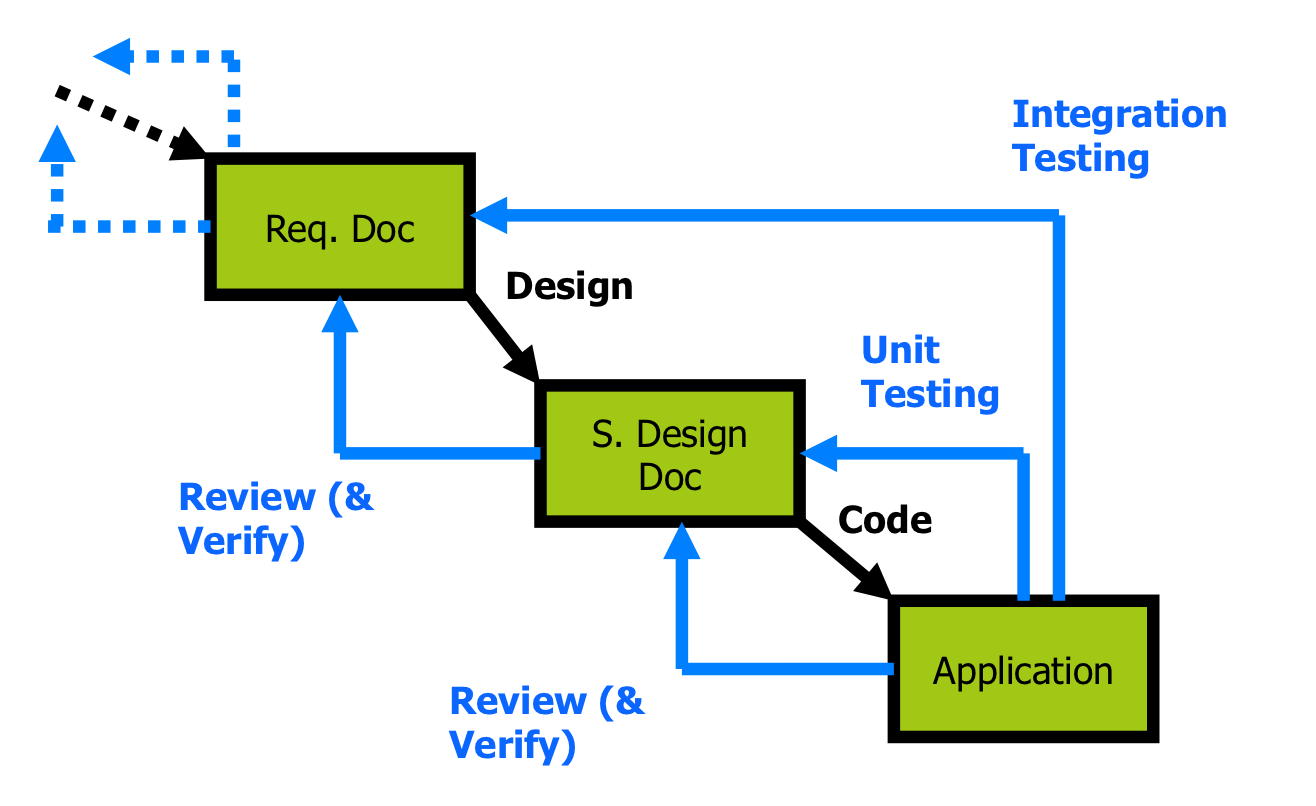
\includegraphics[scale=0.55]{../Figures/SoftwareLifecycle.png}
\end{center}

\end{frame}

%%%%%%%%%%%%%%%%%%%%%%%%%%%%%%%%%%%%%%%%%%%%%%%%%%%%%%%%%%%%%%%%%%%%%%%%%%%%%

\begin{frame}
\frametitle{Testing Phases}
\begin{enumerate}
\item Unit testing
\item Integration testing
\item System testing
\item Acceptance testing
\end{enumerate}
\end{frame}

%%%%%%%%%%%%%%%%%%%%%%%%%%%%%%%%%%%%%%%%%%%%%%%%%%%%%%

\begin{frame}
\frametitle{Need for Verification}

\begin{itemize}

\item Designers are fallible even if they are skilled and follow sound principles
\item We need to build confidence in the software
\item Everything must be verified, every required functionality, every required
  quality, every process, every product, every document
\item For every work product covered in this class we have discussed its verification
\item Even verification itself must be verified

\end{itemize}

\end{frame}

%%%%%%%%%%%%%%%%%%%%%%%%%%%%%%%%%%%%%%%%%%%%%%%%%%%%%%%%%%%%%%%%%%%%%%%%%%%%%

\begin{frame}
\frametitle{Properties of Verification}

From \cite{GhezziEtAl2003}

\begin{itemize}

\item May not be binary (OK, not OK)
\begin{itemize}
\item Severity of defect is important
\item Some defects may be tolerated
\item Our goal is typically acceptable reliability, not correctness
\end{itemize}
\item May be subjective or objective - for instance, usability, generic level of
  maintainability or portability
\bi
\item \structure{How might we make usability objective?}
\ei
\item Even implicit qualities should be verified
\begin{itemize}
\item Because requirements are often incomplete
\item For instance robustness, maintainability
\end{itemize}
\item \structure{What is better than implicitly specified
    qualities?} % explicit!
\end{itemize}

\end{frame}

%%%%%%%%%%%%%%%%%%%%%%%%%%%%%%%%%%%%%%%%%%%%%%%%%%%%%%%%%%%%%%%%%%%%%%%%%%%%%

\begin{frame}
\frametitle{Approaches to Verification}

\begin{itemize}

\item \structure{What are some approaches to verification?}
\item \structure{How can we categorize these approaches?}

\end{itemize}

\end{frame}

%%%%%%%%%%%%%%%%%%%%%%%%%%%%%%%%%%%%%%%%%%%%%%%%%%%%%%%%%%%%%%%%%%%%%%%%%%%%%

\begin{frame}
\frametitle{Approaches to Verification}

\begin{itemize}

\item Experiment with behaviour of product
\begin{itemize}
\item Sample behaviours via testing
\item Goal is to find ``counter examples''
\item \structure{Dynamic} technique
\item Examples: unit testing, integration testing, acceptance testing, white box
  testing, stress testing, etc.
\end{itemize}
\item Analyze product to deduce its adequacy
\begin{itemize}
\item Analytic study of properties
\item \structure{Static} technique
\item Examples: Code walk-throughs, code inspections, correctness proof, etc.
\end{itemize}

\end{itemize}

\end{frame}

%%%%%%%%%%%%%%%%%%%%%%%%%%%%%%%%%%%%%%%%%%%%%%%%%%%%%%%%%%%%%%%%%%%%%%%%%%%%%

\begin{frame}
\frametitle{Does our Engineering Analogy Fail?}

\begin{itemize}

\item \structure{If a bridge can hold 512 kN, can it hold 499 kN?}
\item \structure{If our software works for the input 512, will it work for 499?}

\end{itemize}

\end{frame}

%%%%%%%%%%%%%%%%%%%%%%%%%%%%%%%%%%%%%%%%%%%%%%%%%%%%%%

\begin{frame}
\frametitle{Verification in Engineering}

\begin{itemize}

\item Example of bridge design
\item One test assures infinite correct situations
\item In software a small change in the input may result in significantly different behaviour
\item There are also chaotic systems in nature, but products of engineering
  design are usually stable and well-behaved
% consider the examples of weather, bifurcation in engineering, chaos theory for traffic, etc.
\end{itemize}

\end{frame}

%%%%%%%%%%%%%%%%%%%%%%%%%%%%%%%%%%%%%%%%%%%%%%%%%%%%%%

\begin{frame}
\frametitle{Modified Version Works for 512, but not 499}

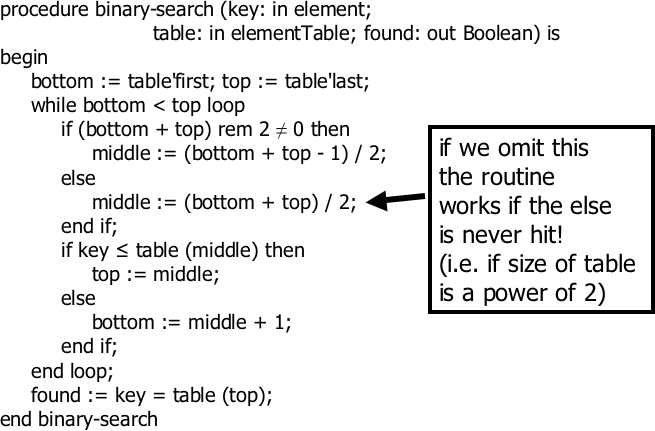
\includegraphics[scale=0.5]{../Figures/BinarySearch.png}

\end{frame}

%%%%%%%%%%%%%%%%%%%%%%%%%%%%%%%%%%%%%%%%%%%%%%%%%%%%%%

\begin{frame}
\frametitle{Testing and Lack of ``Continuity''}

\begin{itemize}

\item Testing samples behaviours by examining ``test cases''
\item Impossible to extrapolate behaviour of software from a finite set of test cases
\item No continuity of behaviour - it can exhibit correct behaviour in
  infinitely many cases, but may still be incorrect in some cases

\end{itemize}

\end{frame}

%%%%%%%%%%%%%%%%%%%%%%%%%%%%%%%%%%%%%%%%%%%%%%%%%%%%%%

\begin{frame}
\frametitle{Goals of Testing}

\begin{itemize}

\item \structure{If our code passes all test cases, is it now guaranteed to be
    error free?}
\item \structure{Are 5000 random tests always better than 5 carefully selected
    tests?}

\end{itemize}

\end{frame}

%%%%%%%%%%%%%%%%%%%%%%%%%%%%%%%%%%%%%%%%%%%%%%%%%%%%%%

\begin{frame}
\frametitle{Goals of Testing}

\begin{itemize}

\item To show the \structure{presence} of bugs (Dijkstra, 1972)
\item If tests do not detect failures, we cannot conclude that software is defect-free
\item Still, we need to do testing - driven by sound and systematic principles
\begin{itemize}
\item Random testing is often not a systematic principle to use
% look at the example from the text, or divide by zero within a circular range
\item Need a test plan
\end{itemize}
\item Should help isolate errors - to facilitate debugging

\end{itemize}

\end{frame}

%%%%%%%%%%%%%%%%%%%%%%%%%%%%%%%%%%%%%%%%%%%%%%%%%%%%%%

\begin{frame}
\frametitle{Goals of Testing Continued}

\begin{itemize}
\item Should be repeatable
\begin{itemize}
\item Repeating the same experiment, we should get the same results
\item Repeatability may not be true because of the effect of the execution
  environment on testing
\item Repeatability may not occur if there are uninitialized variables
\item Repeatability may not happen when there is nondeterminism
\end{itemize}

\item Should be accurate
\begin{itemize}
\item Accuracy increases reliability
\item Part of the motivation for formal specification
\end{itemize}

\item \structure{Is a \structure{successful} test case one that passes the test, or one
  that shows a failure?}

\end{itemize}

\end{frame}

%%%%%%%%%%%%%%%%%%%%%%%%%%%%%%%%%%%%%%%%%%%%%%%%%%%%%%

\begin{frame}
\frametitle{Test (V\&V) Plan}

\begin{itemize}

\item \structure{Given that no single verification technique can prove
    correctness, the practical approach is to use ALL verification techniques.
    Is this statement True or False?}

\end{itemize}

\end{frame}

%%%%%%%%%%%%%%%%%%%%%%%%%%%%%%%%%%%%%%%%%%%%%%%%%%%%%%

\begin{frame}
\frametitle{Test (V\&V) Plan}

\begin{itemize}

\item Testing can uncover errors and build confidence in the software
\item Resources of time, people, facilities are limited
\item Need to plan how the software will be tested
\item You know in advance that the software is unlikely to be perfect
\item You need to put resources into the most important parts of the project
\item A risk analysis can determine where to put your limited resources
\item A risk is a condition that can result in a loss
\item Risk analysis involves looking at how bad the loss can be and at the
  probability of the loss occurring

\end{itemize}

\end{frame}

%%%%%%%%%%%%%%%%%%%%%%%%%%%%%%%%%%%%%%%%%%%%%%%%%%%%%%

\begin{frame}
\frametitle{White Box Versus Black Box Testing}
\begin{itemize}
\item \structure{Do you know (or can you guess) the difference between white box
    and black box testing?}
\item \structure{What if they were labelled transparent box and opaque box
    testing, respectively?}
\end{itemize}
\end{frame}

%%%%%%%%%%%%%%%%%%%%%%%%%%%%%%%%%%%%%%%%%%%%%%%%%%%%%%

\begin{frame}
\frametitle{White Box Versus Black Box Testing}
\begin{itemize}
\item White box testing is derived from the program's internal structure
\item Black box testing is derived from a description of the program's function
\item Should perform both white box and black box testing
\item Black box testing
\begin{itemize}
\item Uncovers errors that occur in implementing requirements or design specifications
\item Not concerned with how processing occurs, but with the results
\item Focuses on functional requirements for the system
\item Focuses on normal behaviour of the system
\end{itemize}
\end{itemize}
\end{frame}

%%%%%%%%%%%%%%%%%%%%%%%%%%%%%%%%%%%%%%%%%%%%%%%%%%%%%%

\begin{frame}
\frametitle{White Box Testing}

\begin{itemize}
\item Uncovers errors that occur during implementation of the program
\item Concerned with how processing occurs
\item Evaluates whether the structure is sound
%\item Focuses on the nonfunctional requirements for the system
\item Focuses on abnormal or extreme behaviour of the system
\end{itemize}

\end{frame}

%%%%%%%%%%%%%%%%%%%%%%%%%%%%%%%%%%%%%%%%%%%%%%%%%%%%%%

\begin{frame}
\frametitle{Dynamic Testing}
\begin{itemize}
\item \structure{Is there a dynamic testing technique that can guarantee
    correctness?}
\item \structure{If so, what is the technique?}
\item \structure{Is this technique practical?}
\end{itemize}
\end{frame}

%%%%%%%%%%%%%%%%%%%%%%%%%%%%%%%%%%%%%%%%%%%%%%%%%%%%%%

\begin{frame}
\frametitle{Dynamic Versus Static Testing}
\begin{itemize}
\item Another classification of verification techniques, as previously discussed
\item Use a combination of dynamic and static testing
\item Dynamic analysis
\begin{itemize}
\item Requires the program to be executed
\item Test cases are run and results are checked against expected behaviour
\item Exhaustive testing is the only dynamic technique that guarantees program
validity
\item Exhaustive testing is usually impractical or impossible
\item Reduce number of test cases by finding criteria for choosing representative test cases
\end{itemize}
\end{itemize}
\end{frame}

%%%%%%%%%%%%%%%%%%%%%%%%%%%%%%%%%%%%%%%%%%%%%%%%%%%%%%

\begin{frame}
\frametitle{Static Testing Continued}
\begin{itemize}
\item Static analysis
\begin{itemize}
\item Does not involve program execution
\item Testing techniques simulate the dynamic environment
\item Includes syntax checking
\item Generally static testing is used in the requirements and design stage, where there is no code to execute
\item Document and code walkthroughs
\item Document and code inspections
\end{itemize}
\end{itemize}
\end{frame}
 
%%%%%%%%%%%%%%%%%%%%%%%%%%%%%%%%%%%%%%%%%%%%%%%%%%%%%%

\begin{frame}
\frametitle{Manual Versus Automated Testing}
\begin{itemize}
\item \structure{What is the difference between manual and automated testing?}
\item \structure{What are the advantages of automated testing?}
\item \structure{What is regression testing?}
\end{itemize}
\end{frame}

%%%%%%%%%%%%%%%%%%%%%%%%%%%%%%%%%%%%%%%%%%%%%%%%%%%%%%

\begin{frame}
\frametitle{Manual Versus Automated Testing}
\begin{itemize}
\item Manual testing
\begin{itemize}
\item Has to be conducted by people
\item Includes by-hand test cases, structured walkthroughs, code inspections
\end{itemize}
\item Automated testing
\begin{itemize}
\item The more automated the development process, the easier to automate testing
\item Less reliance on people
\item Necessary for \structure{regression testing}
\item Test tools can assist, such as Junit, Cppunit, CuTest etc.
\item Can be challenging to automate GUI tests
\item Test suite for Maple has 2 000 000 test cases, run on 14 platforms, every
  night, automated reporting
\end{itemize}
\end{itemize}
\end{frame}

%%%%%%%%%%%%%%%%%%%%%%%%%%%%%%%%%%%%%%%%%%%%%%%%%%%%%%

% \begin{frame}
% \frametitle{Automated Testing at MapleSoft}
% \begin{itemize}
% \item Three steps
% \begin{itemize}
% \item Write the problem description
% \item result := solver(problem)
% \item assert(result == expected)
% \end{itemize}
% \item Assert writes out code to reproduce any failures
% \item Track failures
% \begin{itemize}
% \item Source code management (like CVS or Subversion)
% \item Database of test cases, functions called
% \item Database of source files, functions defined
% \item Database of 40 days of timings and resources used
% \end{itemize}
% \item Automatically sends an e-mail to the programmer and his/her boss
% \end{itemize}
% \end{frame}

% %%%%%%%%%%%%%%%%%%%%%%%%%%%%%%%%%%%%%%%%%%%%%%%%%%%%%%

\begin{frame}
\frametitle{Continuous Integration Testing}
\begin{itemize}
\item \structure{What is continuous integration testing?}
\end{itemize}
\end{frame}

%%%%%%%%%%%%%%%%%%%%%%%%%%%%%%%%%%%%%%%%%%%%%%%%%%%%%%

\begin{frame}
\frametitle{Continuous Integration Testing}
\begin{itemize}
\item Information available on
  \href{https://en.wikipedia.org/wiki/Continuous_integration}{Wikipedia}
\item Developers integrate their code into a shared repo frequently (multiple
  times a day)
\item Each integration is automatically accompanied by regression tests and
  other build tasks
\item Build server
\bi
\item Unit tests
\item Integration tests
\item Static analysis
\item Profile performance
\item Extract documentation
\item Update project web-page
\item Portability tests
\item etc.
\ei
\item Avoids potentially extreme problems with integration when the baseline and
  a developer's code greatly differ
\end{itemize}
\end{frame}

%%%%%%%%%%%%%%%%%%%%%%%%%%%%%%%%%%%%%%%%%%%%%%%%%%%%%%

\begin{frame}
\frametitle{Continuous Integration Tools}
\begin{itemize}
\item Gitlab
\bi
\item Example at
  \href{https://gitlab.cas.mcmaster.ca/andrem5/RogueReborn/pipelines}{Rogue
    Reborn}
\ei
\item Jenkins
\item Travis
\item \href{https://www.docker.com/}{Docker}
\bi
\item Eliminates the ``it works on my machine'' problem
\item Package dependencies with your apps
\item A container for lightweight virtualization
\item Not a full VM
\ei
\end{itemize}
\end{frame}

%%%%%%%%%%%%%%%%%%%%%%%%%%%%%%%%%%%%%%%%%%%%%%%%%%%%%%

\begin{frame}
\frametitle{Sample Nonfunctional System Testing}
\begin{itemize}
\item Stress testing - Determines if the system can function when subject to large volumes
\item Usability testing
\item Performance measurement
\end{itemize}
\end{frame}

%%%%%%%%%%%%%%%%%%%%%%%%%%%%%%%%%%%%%%%%%%%%%%%%%%%%%%

\begin{frame}
\frametitle{Sample Functional System Testing}
\begin{itemize}
\item Requirements: Determines if the system can perform its function correctly and that the correctness can be
sustained over a continuous period of time
%\item Regression: Determines if changes to the system do not invalidate previous positive testing results
\item Error Handling: Determines the ability of the system to properly process
  incorrect transactions
\item Manual Support: Determines that the manual support procedures are documented and complete, where manual support
involves procedures, interfaces between people and the system, and training procedures
\item Parallel: Determines the results of the new application are consistent with the processing of the previous
application or version of the application
\end{itemize}
\end{frame}

%%%%%%%%%%%%%%%%%%%%%%%%%%%%%%%%%%%%%%%%%%%%%%%%%%%%%%

\begin{frame}
\frametitle{Theoretical Foundations Of Testing: Definitions}
\begin{itemize}
\item P (program), D (input domain), R (output domain)
\bi
\item P: D $\rightarrow$ R (may be partial)
\ei
\item Correctness defined by OR $\subseteq$ D $\times$ R
\bi
\item P(d) correct if $\langle$ d, P(d) $\rangle \in$ OR
\item P correct if all P(d) are correct
\ei
\item Failure
\bi
\item P(d) is not correct
\item May be undefined (error state) or may be the wrong result
\ei
\item Error (Defect)
\bi
\item Anything that may cause a failure
\bi
\item Typing mistake
\item Programmer forgot to test ``x=0''
\ei
\ei
\item Fault
\bi
\item Incorrect intermediate state entered by program
\ei
\end{itemize}
\end{frame}

%%%%%%%%%%%%%%%%%%%%%%%%%%%%%%%%%%%%%%%%%%%%%%%%%%%%%%

\begin{frame}
\frametitle{Definitions Questions}
\begin{itemize}
\item \structure{A test case t is an element of D or R?}
\item \structure{A test set T is a finite subset of D or R?}
\item \structure{How would we define whether a test is successful?}
\item \structure{How would we define whether a test set is successful?}
\end{itemize}
\end{frame}

%%%%%%%%%%%%%%%%%%%%%%%%%%%%%%%%%%%%%%%%%%%%%%%%%%%%%%

\begin{frame}
\frametitle{Definitions Continued}
\begin{itemize}
\item Test case t: An element of D
\item Test set T: A finite subset of D
\item Test is successful if P(t) is correct
\item Test set successful if P correct for all t in T
\end{itemize}
\end{frame}

%%%%%%%%%%%%%%%%%%%%%%%%%%%%%%%%%%%%%%%%%%%%%%%%%%%%%%

\begin{frame}
\frametitle{Theoretical Foundations of Testing}

\begin{itemize}
\item Desire a test set $T$ that is a finite subset of $D$ that will uncover all errors
\item Determining and ideal $T$ leads to several
  \href{https://en.wikipedia.org/wiki/Undecidable_problem}{undecideable
    problems}
\item No algorithm exists:
\bi
\item To state if a test set will uncover all possible errors
\item To derive a test set that would prove program correctness
\item To determine whether suitable input exists to guarantee execution of a
  given statement in a given program
\item etc.
\ei
\end{itemize}

\end{frame}

%%%%%%%%%%%%%%%%%%%%%%%%%%%%%%%%%%%%%%%%%%%%%%%%%%%%%%

\begin{frame}
\frametitle{Empirical Testing}

\begin{itemize}
\item Need to introduce empirical testing principles and heuristics as a
  compromise between the impossible and the inadequate
\item Find a strategy to select \structure{significant} test cases
\item Significant means the test cases have a high potential of uncovering the
  presence of errors
\end{itemize}

\end{frame}

%%%%%%%%%%%%%%%%%%%%%%%%%%%%%%%%%%%%%%%%%%%%%%%%%%%%%%

\begin{frame}
\frametitle{Complete-Coverage Principle}

\begin{itemize}
\item Try to group elements of $D$ into subdomains $D_1$, $D_2$, ..., $D_n$
  where any element of each $D_i$ is likely to have similar behaviour
\item $D = D_1 \cup D_2 \cup ... \cup D_n$
\item Select one test as a representative of the subdomain
\item If $D_j \cap D_k = \emptyset$ for all $j \neq k$, (partition), any element
  can be chosen from each subdomain
\item Otherwise choose representatives to minimize number of tests, yet
  fulfilling the principle
\end{itemize}

\end{frame}

%%%%%%%%%%%%%%%%%%%%%%%%%%%%%%%%%%%%%%%%%%%%%%%%%%%%%%

\begin{frame}
\frametitle{Complete-Coverage Principle}

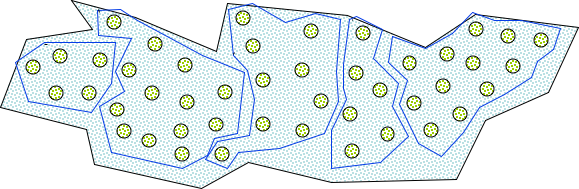
\includegraphics[scale=0.5]{../Figures/CompleteCoveragePrinciple.png}

\end{frame}

%%%%%%%%%%%%%%%%%%%%%%%%%%%%%%%%%%%%%%%%%%%%%%%%%%%%%%

\begin{frame}[allowframebreaks]
\frametitle{References}

\bibliography{../../ReferenceMaterial/References}

\end{frame}

%%%%%%%%%%%%%%%%%%%%%%%%%%%%%%%%%%%%%%%%%%%%%%%%%%%%%%

\end{document}